
\begin{figure}[t]
    \centering

    \subfloat[
        Diagram provided to students to illustrate transitioning between privilege modes (from \enquote{RISC-V Bytes: Privilege Levels} by Daniel Mangum \cite{danielmangumRISCVPriv})
    ]{
        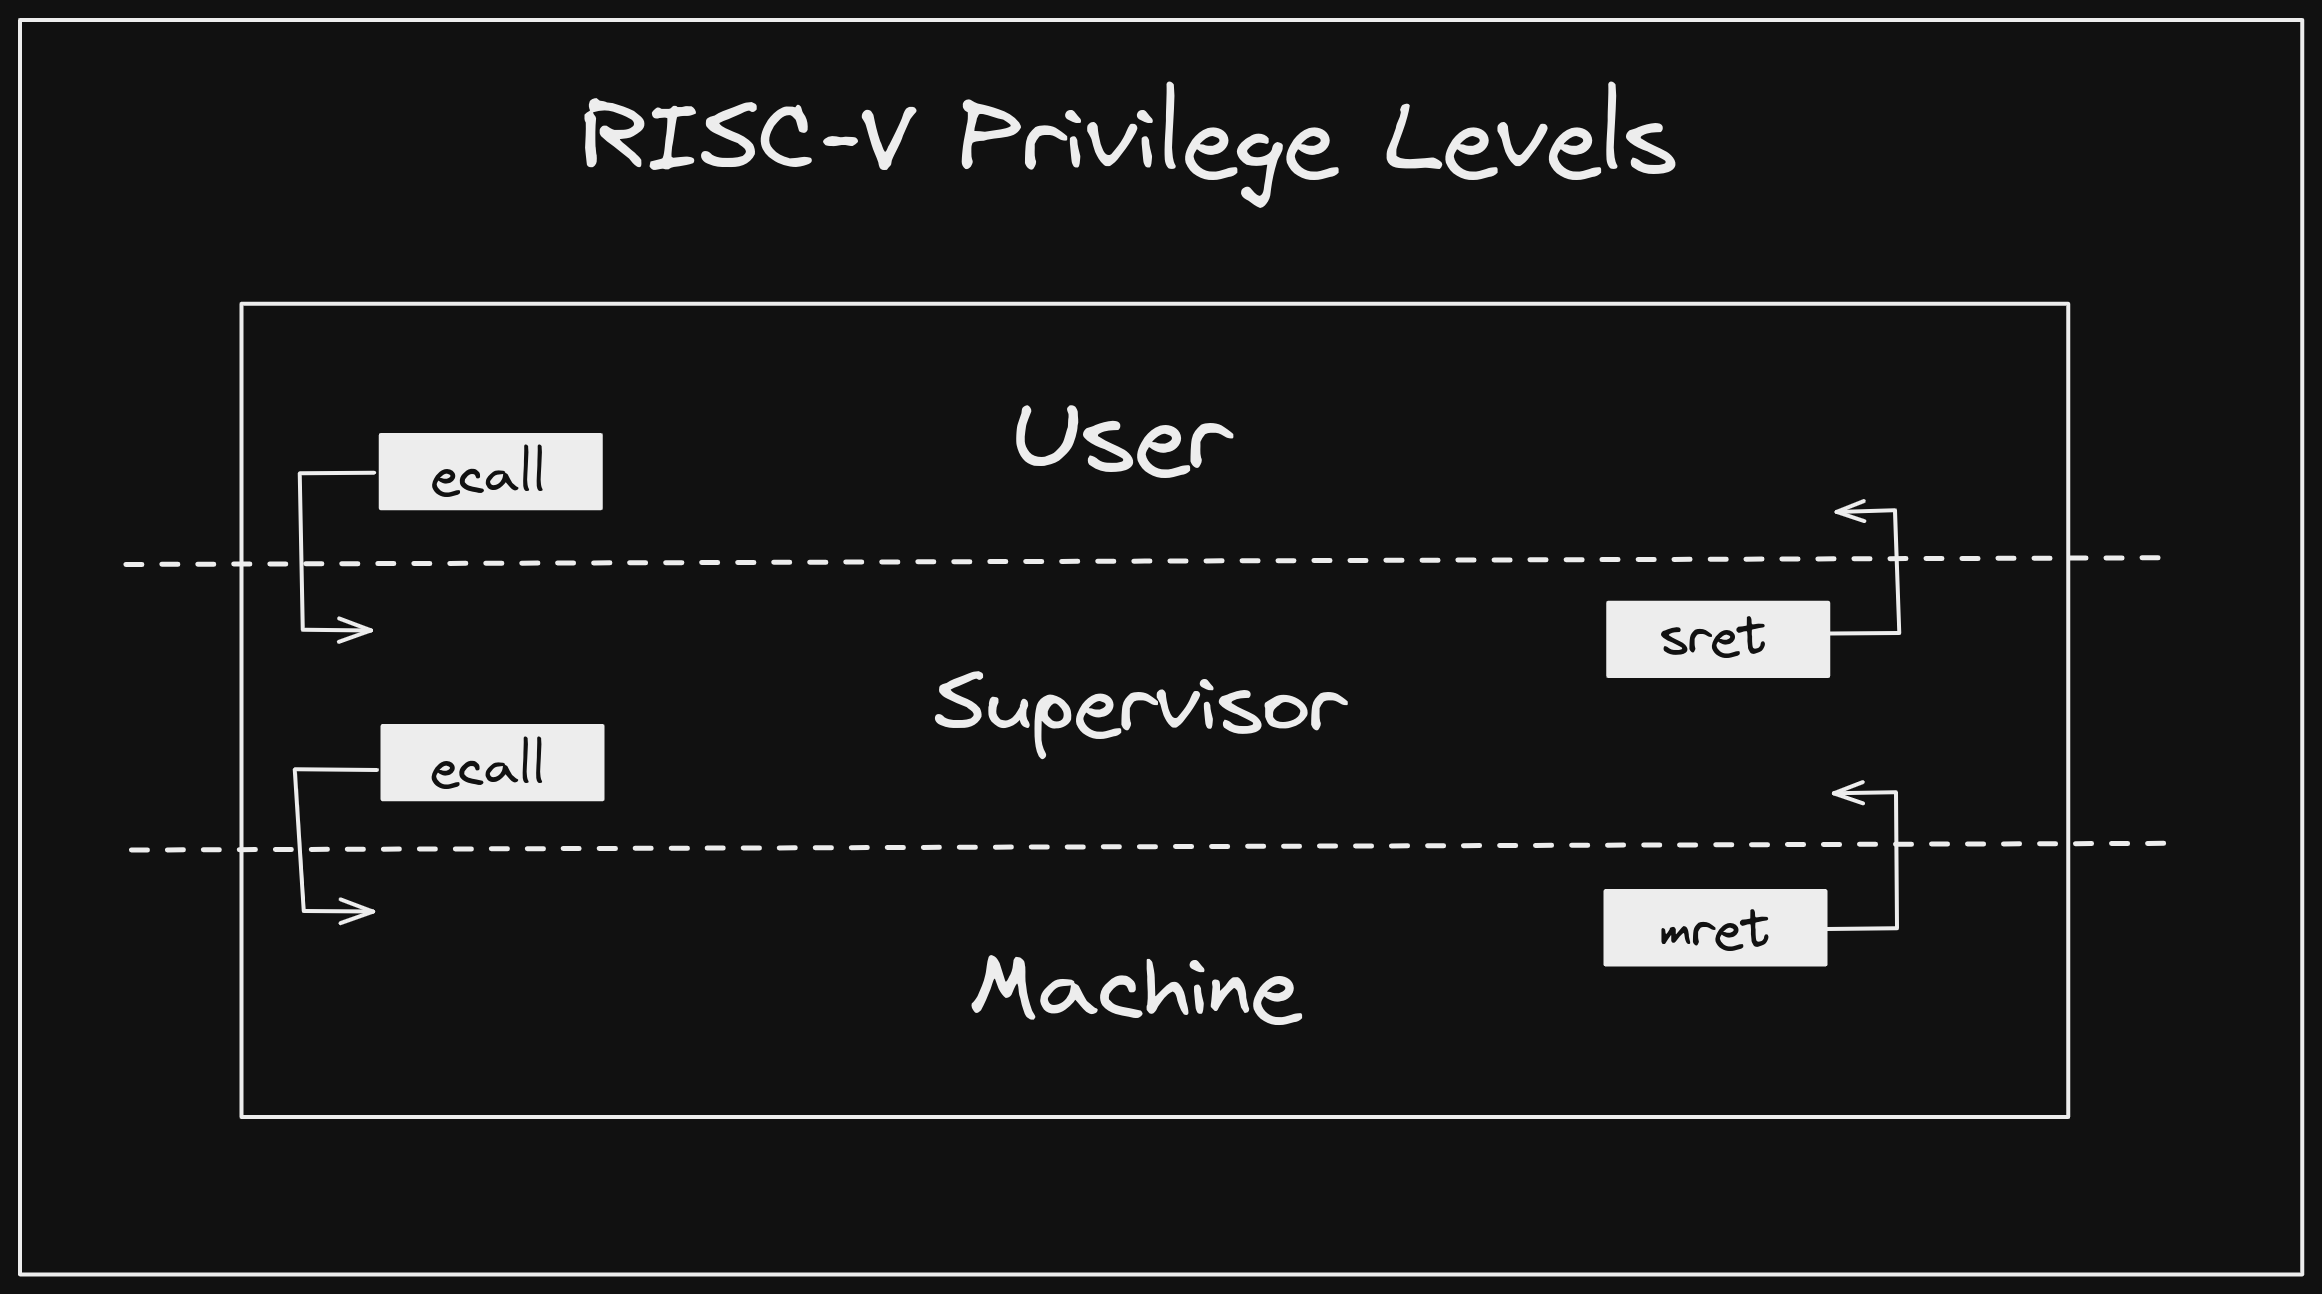
\includegraphics[width=0.9\linewidth]{media/graphics/labs_with_cva6/priv_levels.png}
    }

    \subfloat[
        Page table diagram of provided OS \emph{(student submission)}
    ]{
        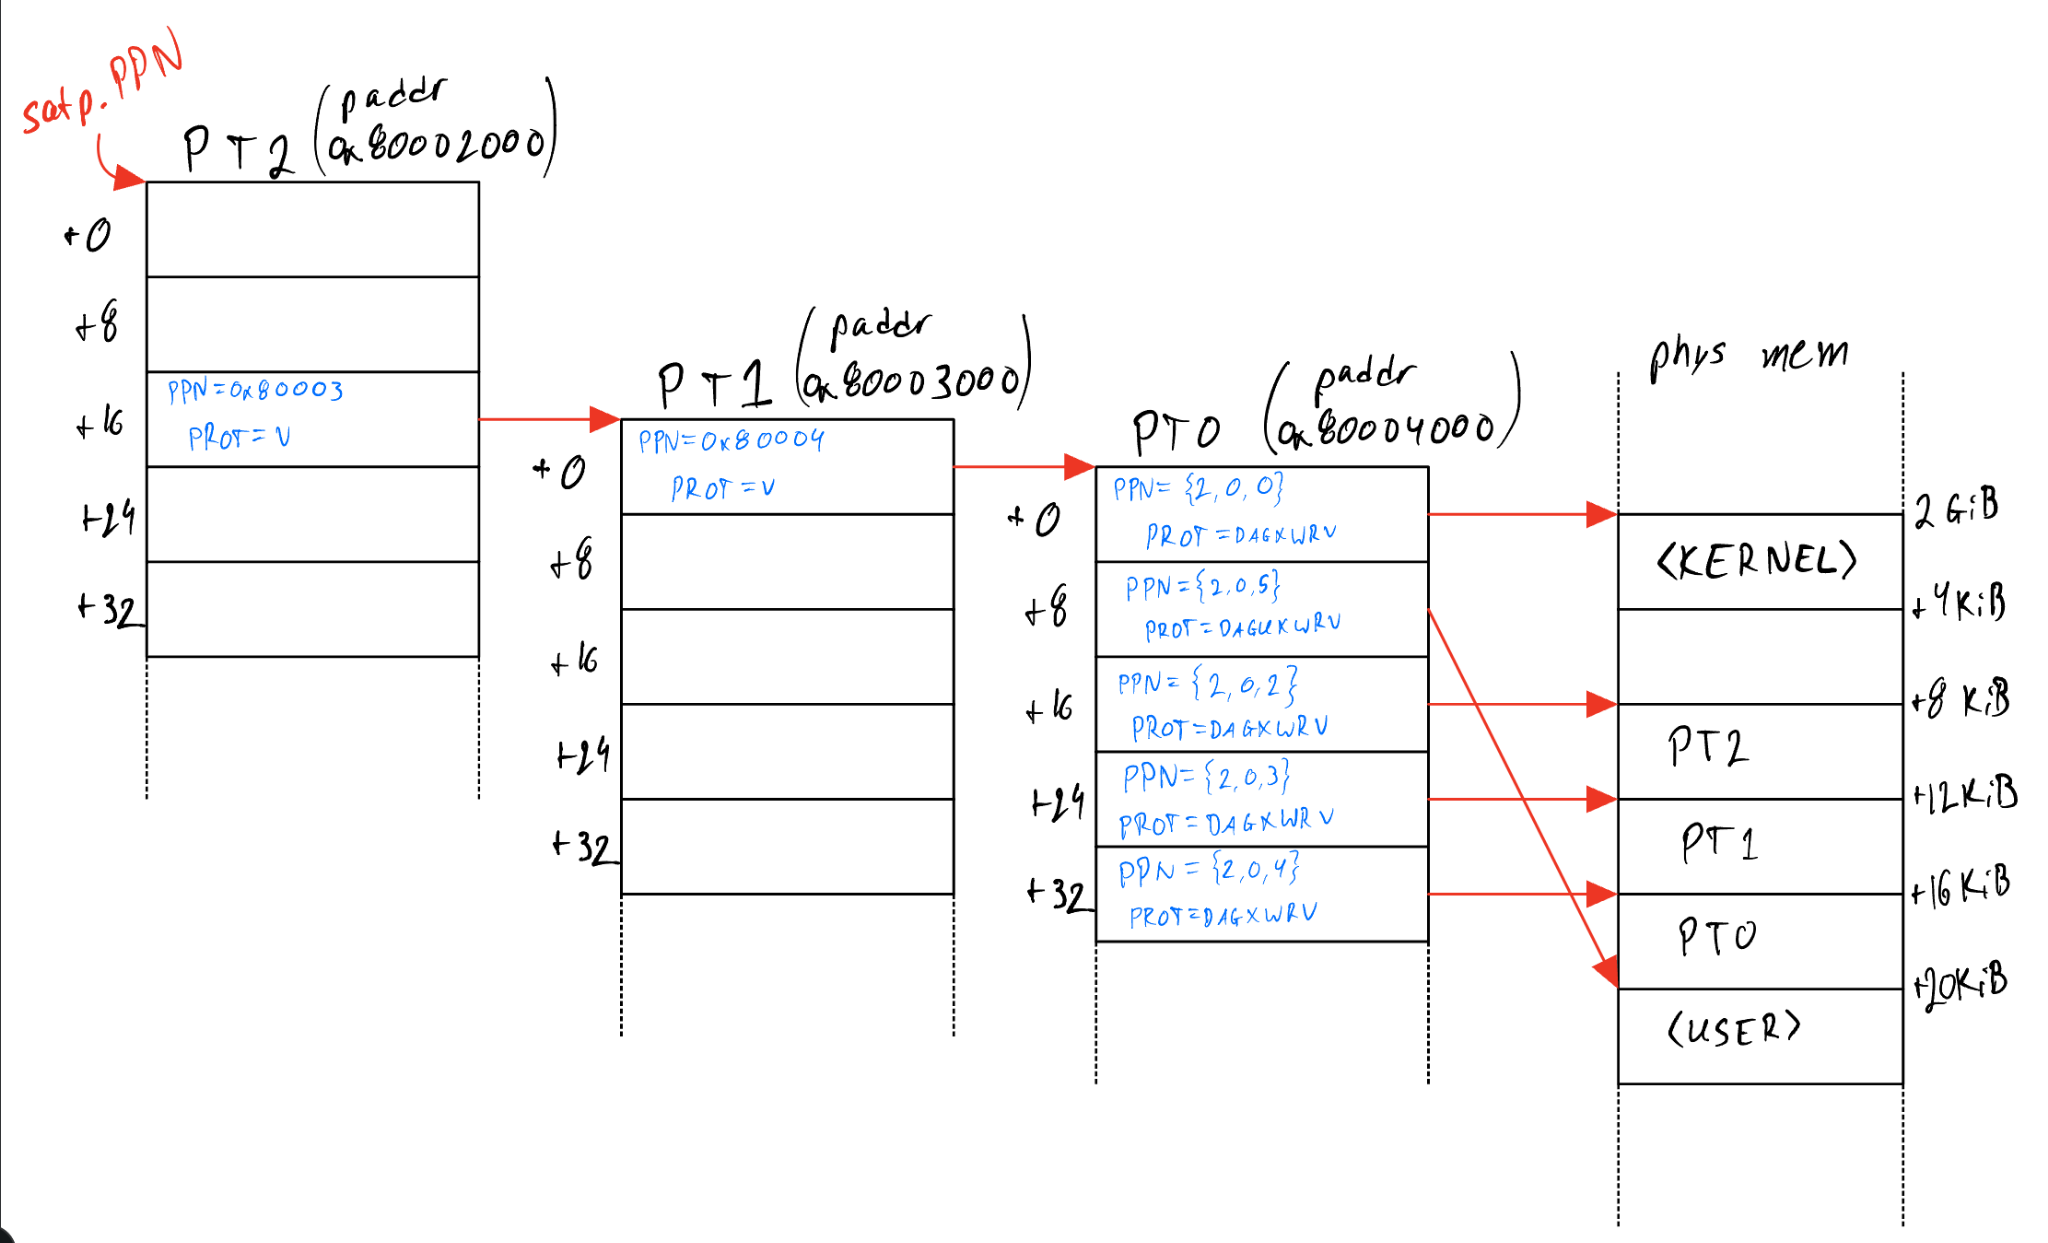
\includegraphics[width=0.9\linewidth]{media/graphics/labs_with_cva6/pt.png}
    }

    \caption[
        Virtual Memory Lab
    ]{
        The Virtual Memory Lab aids students in understanding concepts such as physical vs. virtual memory, page tables, privilege levels, and trap handling in RISC-V architecture.
    }
    \label{fig:virtual_memory}

\end{figure}
